\section{\label{III-C-2}Entraîner une IA sur la base d’un vocabulaire spécialisé : défis et solutions}

Cette ambition d’automatiser le traitement des thésaurus se heurte, au MAE, à des contraintes majeures. Ce musée, sous tutelle du \minarm, ne saurait exposer ses données sensibles -- notices techniques, archives, référentiels -- à des modèles externes ou à des services cloud\footnote{A ce sujet, les support informatique du musée se conforme autant que possible aux recommandations de l'\ac{anssi}, et à la suite des méfiances exprimées par l'organisme concernant la sécurité et la confidentialité des données d'entraînement des \ac{llm}, la nouvelle charte informatique de septembre 2025 demandera à tous les agents de s'engager à ne pas les utiliser.}. La confidentialité, renforcée par le \ac{rgpd} et les restrictions propres au secteur, impose une politique de sécurité stricte : tout entraînement doit s’effectuer sur des outils déployés en interne, sur serveurs sécurisés, sans échange hors du périmètre institutionnel.

La méthodologie proposée lors de ce stage pour entraîner une IA sur les vocabulaires spécialisés du musée tente de faire face à ces contraintes. L’entraînement à partir de Wikidata, par extraction du vocabulaire aéronautique via requêtes SPARQL\footnote{Cf. [TODO annexe]}, permet de sélectionner des concepts pertinents, mais génère un bruit considérable : l'exhaustivité reste partielle, et il est difficile de ne pas récupérer de termes non pertinents ce qui nécessite un nettoyage manuel important.

Une autres difficulté rencontrée est le manque de précédent sur des projets de ce type : si les projets d'implémentation de l'\ac{ia} pour des tâches d'indexation -- où celle-ci peut donc mettre chaque oeuvre dans un contexte, de contenu ou de description --, aucun précédent d'utilisation pour traiter un thésaurus semble n'avoir été réalisé, ou du moins diffusé sur le web. La tâche est en effet complexe : dans un thésaurus, chaque mot est indépendant, et il comprend peu de matière de contextualisation dont un modèle de type \textit{bert}\footnote{voir paragraphe précédent} aurait besoin. La solution semble donc être l'utilisation d'un \ac{llm} : cependant, ceux-ci peinent à saisir les nuances du vocabulaire extrêmement spécialisé utilisé par le musée. La solution qui a donc été proposée est l'entraînement d'un \ac{llm} en local\footnote{des tests encore peu concluant ont été réalisés avec le modèle \textit{llama3:2}} sur les données extraites de Wikidata -- dont les termes sont déjà définis et associés entre eux -- et un corpus de données du musée avant de lui fournir les fichiers csv des thésaurus du musée pour lui demander de reconnaître d'éventuels synonymes, associations, et hiérarchisations\footnote{[TODO : ajout annexe prompt et modèle]}. 

\begin{figure}[htbp]
	\centering
	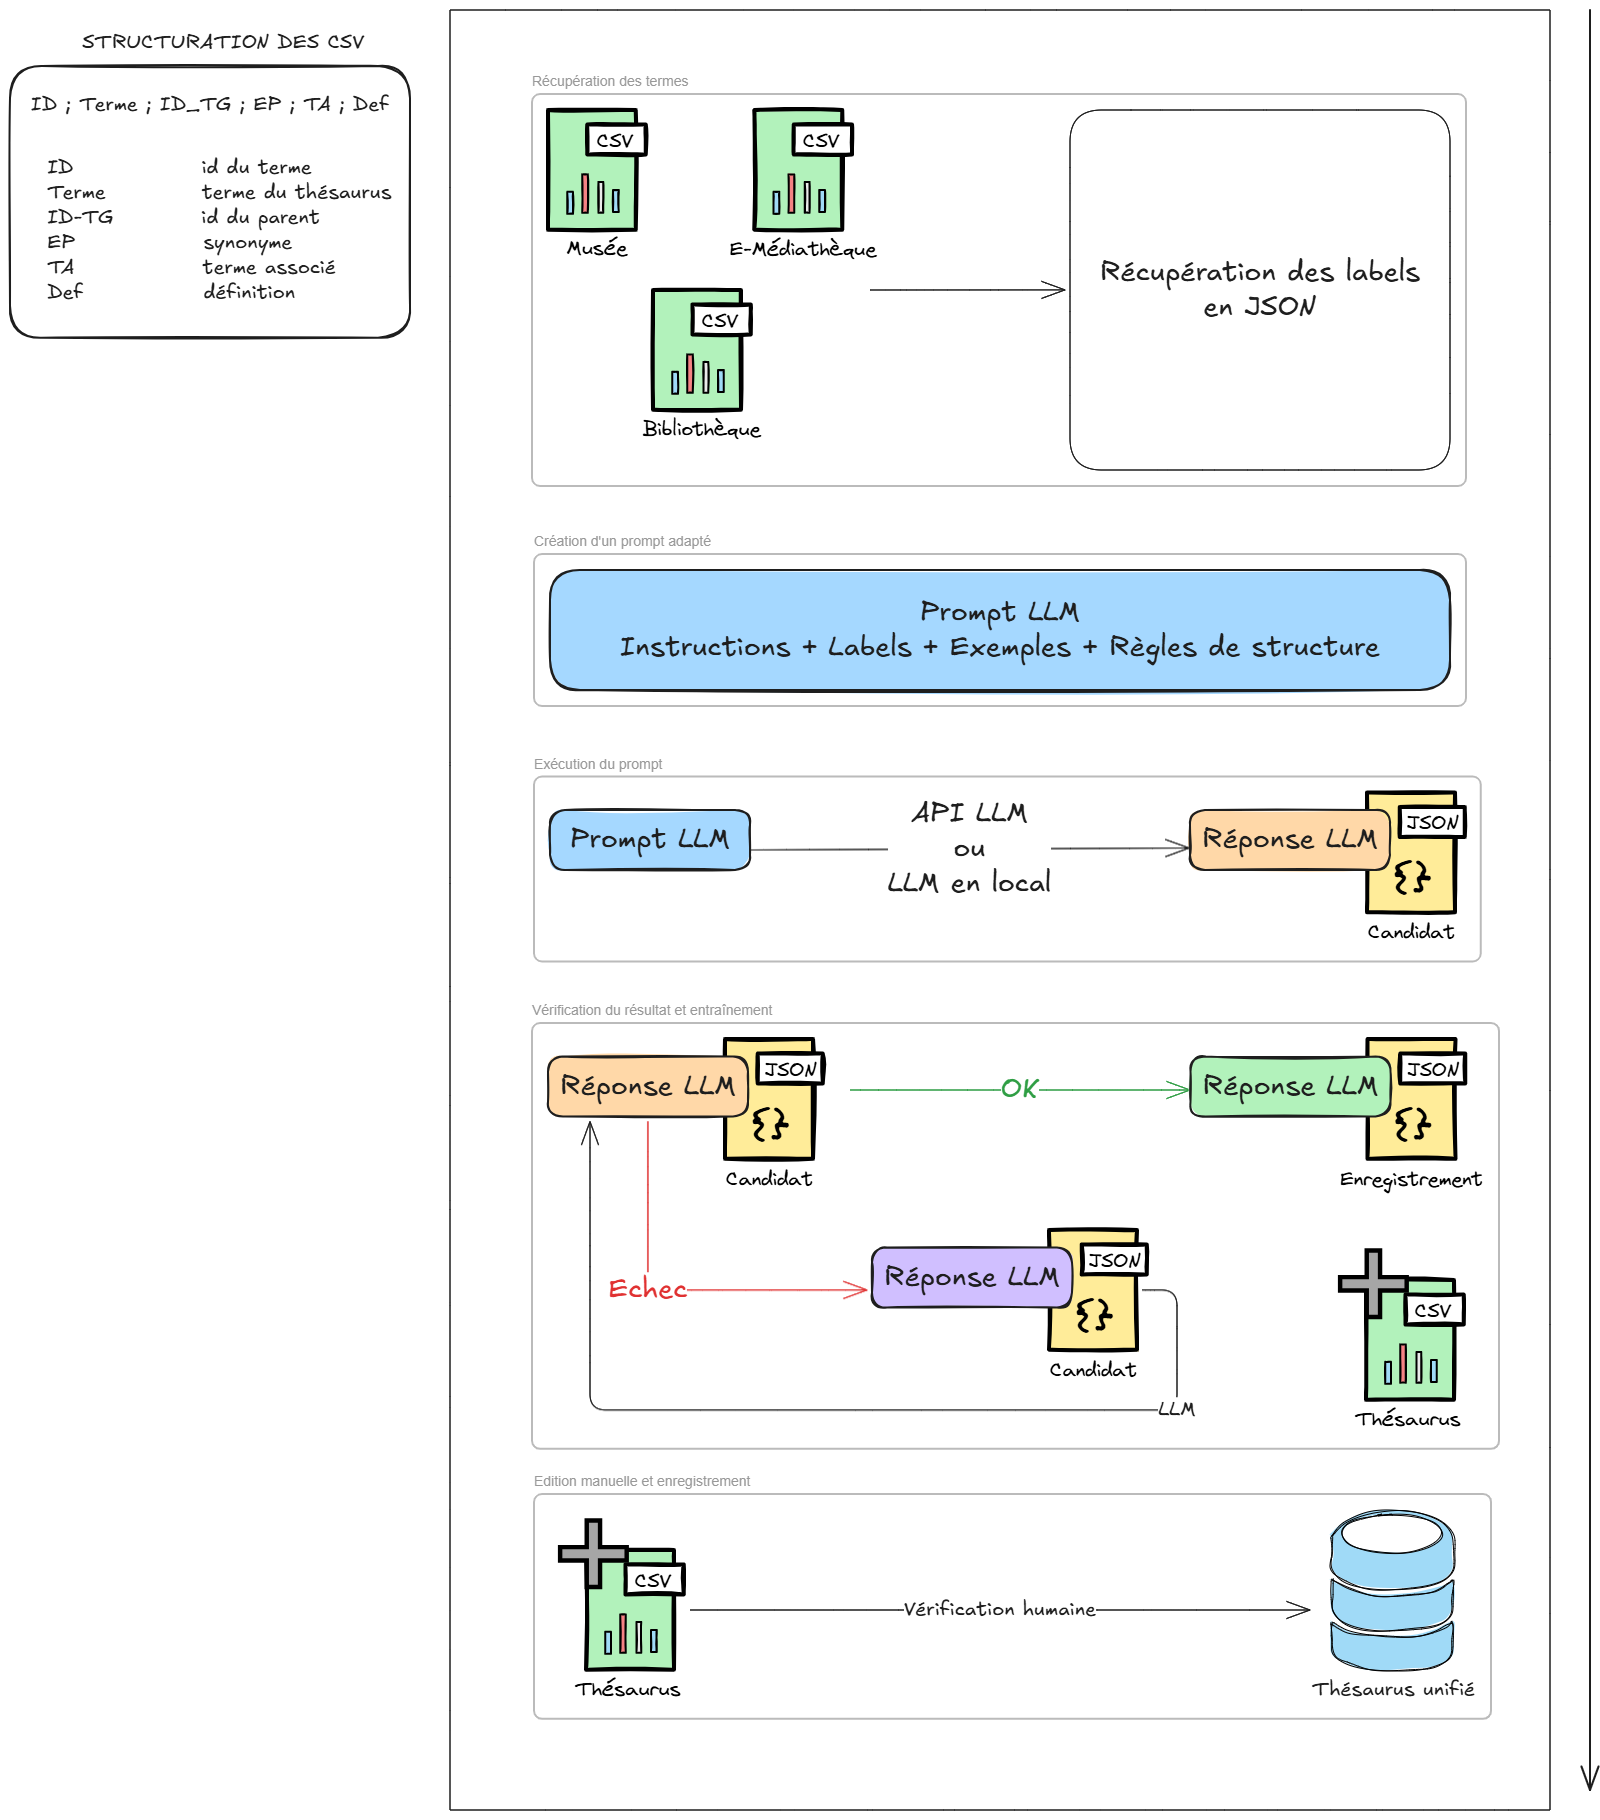
\includegraphics[width=0.7\linewidth]{img/SCHEM_processus_IA}
	\caption[Proposition de processus d'implémentation d'une IA au \mae]{Proposition de processus d'implémentation d'une IA au \mae~après entraînement sur un corpus spécialisé.}
	\label{fig:schemprocessusia}
\end{figure}



\paragraph*{Limites et perspectives}
À ce stade cependant, demeure la limite de la spécialisation du vocabulaire du musée : même si l'\ac{ia} peut permettre d'alléger la charge de travail des agents travaillant à l'unification du thésaurus, une validation humaine reste nécessaire, pour entraîner l'\ac{ia} et valider ses données. Ceci demande donc de mettre en place une pratique hybride qui articulerait automatisation et savoir-faire documentaire, avant d'aligner le résultat sur des formats \ac{skos}/\ac{rdf}, dans le respect des contraintes propres au musée.

La réflexion sur l’apport de l’IA en institution patrimoniale ne se résume pas à une question d’outillage : elle engage en effet un débat sur la gouvernance de l’information et sur la capacité de l’institution à transmettre son patrimoine sans le dissoudre dans l’automatisme. L'\ac{ia}, ici comme ailleurs, ne reste utile que si elle demeure un auxiliaire du métier et non un substitut. 